\chapter{Zener Diode-Voltage Regulator}
	\section{Aim}
		\begin{itemize}
			\tightlist
			\item Explain the function of a Zener diode
			\item Explain Zener Diode as Voltage Regulator
		\end{itemize}
	
	\section{Apparatus}
		\begin{itemize}
			\tightlist
			\item Zener Diode
			\item Resistors
			\item Ammeter
			\item Voltmeter
			\item DC Battery Source
		\end{itemize}
	
	\section{Theory}
		\subsection{Zener Diode}
			A Zener Diode is a special kind of diode which permits current to flow in the forward direction as normal, but will also allow it to flow in the reverse direction when the voltage is above the breakdown voltage or ‘zener’ voltage. Zener diodes are designed so that their breakdown voltage is much lower - for example just 2.4 Volts.
			\begin{figure}[ht]
				\centering 
				\subfloat[Zener Diode]{\includegraphics[width=0.45\textwidth]{img/exp8/1}
					\label{fig:zener_pic}}
				\hfill
				\subfloat[Symbol of Zener Diode]{\includegraphics[width=0.45\textwidth,valign=c]{img/exp8/2}
					\label{fig:zener_symbol}}
				\caption{\textit{Zener Diode image and symbol}}
			\end{figure}
		
		\subsection{Function of Zener Diode}
			\begin{enumerate}
				\item Zener diodes are a special kind of diode which permits current to flow in the forward direction.
				\item Zener diodes will also allow current to flow in the reverse direction when the voltage is above a certain value. This breakdown voltage is known as the Zener voltage. In a standard diode, the Zener voltage is high, and the diode is permanently damaged if a reverse current above that value is allowed to pass through it.
				\item In the reverse bias direction, there is practically no reverse current flow until the breakdown voltage is reached. When this occurs there is a sharp increase in reverse current. Varying amount of reverse current can pass through the diode without damaging it. The breakdown voltage or zener voltage (\(V_Z\)) across the diode remains relatively constant. 
			\end{enumerate}
		
		\subsection{Zener Diode As A Voltage Regulator}
			A voltage regulator is an electronic circuit that provides a stable DC voltage independent of the load current, temperature and AC line voltage variations. A Zener diode of break down voltage \(V_Z\) is reverse connected to an input voltage source \(V_I\) across a load resistance \(R_L\) and a series resistor \(R_S\). The voltage across the zener will remain steady at its break down voltage \(V_Z\) for all the values of zener current \(I_Z\)  as long as the current remains in the break down region. Hence a regulated DC output voltage \(V_0 = V_Z\) is obtained across \(R_L\), whenever the input voltage remains within a minimum and maximum voltage. Basically there are two type of regulations such as:
			
			\textbf{Line Regulation}: In this type of regulation, series resistance and load resistance are fixed, only input voltage is changing. Output voltage remains the same as long as the input voltage is maintained above a minimum value.
			
			\textbf{Load Regulation}: In this type of regulation, input voltage is fixed and the load resistance is varying. Output volt remains same, as long as the load resistance is maintained above a minimum value.
			
			\subsubsection{Line Regulation}
				\begin{figure}[h]
					\centering
					\includegraphics[width=0.5\linewidth]{img/exp8/3}
					\caption{Zener Diode for Line Regulation}
					\label{fig:zener_lineRegulation}
				\end{figure}
				In Line Regulation, Load resistance is constant and input voltage varies. \(V_I\) must be sufficiently large to turn the Zener Diode ON.
				$$V_L = V_Z= \frac{V_{Imin} \times R_L}{(R_S + R_L)}$$
				So, the minimum turn-on voltage \(V_{Imin}\) is :
				$$ V_{Imin}= \frac{V_Z \times (R_S + R_L)}{R_L}$$
				
				The maximum value of \(V_I\) is limited by the maximum zener current \(I_{Zmax}\)
				$$I_{Rmax}= I_{Zmax} + I_L $$
				
				\(I_L\) is fixed at :
				$$\frac{V_Z}{R_L} \qquad Since, V_L=V_Z $$
				
				So maximum \(V_I\) is
				$$ V_{Imax} = V_{Rmax} + V_Z$$
				or,
				$$V_{Imax} = I_{Rmax} \times R + V_Z$$
				
				For \(V_I < V_Z\),
				$$ V_O= V_I$$
				
				For \(V_I > V_Z\),
				$$ V_O = V_I − I_S \times R_S$$
			
			\subsection{Load Regulation}
				\begin{figure}[h]
					\centering
					\includegraphics[width=0.5\linewidth]{img/exp8/4}
					\caption{Zener Diode for Load Regulation}
					\label{fig:zener_loadRegulation}
				\end{figure}
				In Load Regulation , input voltage is constant and Load resistance varies. Too small a Load Resistance \(R_L\) ,will result in \(V_{Th} < V_Z\) and Zener Diode will be OFF.
				$$V_L = V_Z = \frac{V_{Imin} \times R_L}{(R_S + R_L)}$$
				
				So the minimum load resistance \(R_L\)
				$$R_{Lmin} = \frac{V_Z \times R_S}{V_I− V_Z}$$
				
				Any load resistance greater than \(R_{Lmin}\) will make Zener Diode ON
				$$ I_S = I_L + I_Z$$
				
				\(R_{Lmin}\) will establish maximum \(I_L\) as
				$$I_{Lmax}=\frac{V_L}{R_{Lmin}}= \frac{V_Z}{R_{Lmin}} \qquad Since, V_L=V_Z$$
				
				\(V_S\)is the voltage drop across \(R_S\)
				$$V_S = V_{Imin} - V_Z$$
				$$I_S = \frac{V_{Imin}− V_Z}{R_S}$$
				
				For \(R_L\) < \(R_{Lmin}\),
				$$V_O= V_I$$
				
				For \(R_L\) > \(R_{Lmin}\),
				$$V_O = V_I − I_S \times R_S$$
			
		\section{Procedure}
			\subsection{Zener Diode - Line Regulation}
				\begin{enumerate}
					\tightlist
					\item Set the Zener Voltage($V_Z$)
					\item Set the Series Resistance ($R_S$) value.
					\item Set the Load Resistance ($R_L$) value.
					\item Vary DC voltage.
					\item Voltmeter is placed parallel to load resistor and ammeter series with the series resistor.
					\begin{figure}[h]
						\centering
						\includegraphics[width=0.5\linewidth]{img/exp8/5}
						\caption{Simulation of Zener Diode for Line Regulation}
						\label{fig:zener_Procedure_lineRegulation}
					\end{figure}
					\item Choose appropriate DC voltage such that zener diode is 'on'.
					\item Now note the Voltmeter and Ammeter reading for various DC voltage.
					\item Note the Load current($I_L$), zener current($I_Z$), Output voltage($V_O$)
					\item Calculate the voltage regulation.
				\end{enumerate}
			
			\subsection{Zener Diode - Load Regulation}
				\begin{enumerate}
					\tightlist
					\item Set DC voltage.
					\item Set the Series Resistance ($R_S$) value.
					\item 1W D0-41 Glass Zener Diode 1N4740A, Zener voltage is 10 V.
					\item Vary the Load Resistance ($R_L$).
					\item Voltmeter is placed parallel to load resistor and ammeter series with the series resistor.
					\begin{figure}[h]
						\centering
						\includegraphics[width=0.5\linewidth]{img/exp8/6}
						\caption{Simulation of Zener Diode for Load Regulation}
						\label{fig:zener_Procedure_loadRegulation}
					\end{figure}
					\item Choose Load Resistance in such a manner, such that the Zener diode is 'on'.
					\item Now note the Voltmeter and Ammeter reading for various Load Resistance.
					\item Increase the load resistance ($R_L$).
					\item Note the Load current($I_L$), zener current($I_Z$), Output voltage($V_O$)
					\item Calculate the voltage regulation.
				\end{enumerate}
			
			\subsection{Zener Characteristics}
				\begin{enumerate}
					\tightlist
					\item Select the diode.
					\item Set the rheostat $R_h=1\Omega$
					\item By adjusting the rheostat, voltmeter reading is increased from 0 and in each time note the corresponding reading in milliammeter.
					\begin{figure}[h]
						\centering
						\includegraphics[width=0.5\linewidth]{img/exp8/7}
						\caption{Circuit using Zener Diode for knowing its Characteristics}
						\label{fig:zener_Procedure_charac}
					\end{figure}
					\item Take the readings and note Voltmeter reading across Zener diode and Ammeter reading.
					\item Plot the V-I graph and observe the change.
				\end{enumerate}
		
		\section{Observations}
			\subsection{Zener Diode - Line Regulator}
			Zener Voltage ($V_{Z}$): $5.1 V$\\
			Series Resistance($R_{S}$): $1 K\Omega$\\
			Load Resistance ($R_L$): $2 K\Omega$
			
			\begin{figure}[h!]
				\begin{longtable}[]{@{}llllll@{}}
					\toprule
					Sr No. & UnRegulated & Load & Zener & Regulated & \% Voltage\tabularnewline
					& Supply Voltage & Current & Current & Output Voltage & Regulation\tabularnewline
					& ($V_S$) (V) & ($I_L$) (mA) & ($I_Z$)(mA) & ($V_O$) (V) & \tabularnewline
					\midrule
					\endhead
					1 & 0 & 2.55 & 0 & 0 & NaN\tabularnewline
					2 & 2.4 & 2.55 & 0 & 2.4 & 100\tabularnewline
					3 & 5.6 & 2.55 & -2.050 & 5.10 & 100\tabularnewline
					4 & 9.6 & 2.55 & 1.950 & 5.10 & 55.6\tabularnewline
					5 & 12.8 & 2.55 & 5.150 & 5.10 & 41.7\tabularnewline
					6 & 16 & 2.55 & 8.350 & 5.10 & 31.3\tabularnewline
					7 & 18.2 & 2.55 & 10.550 & 5.10 & 27.8\tabularnewline
					8 & 22 & 2.55 & 14.350 & 5.10 & 22.7\tabularnewline
					9 & 26 & 2.55 & 18.350 & 5.10 & 19.2\tabularnewline
					10 & 29.2 & 2.55 & 21.550 & 5.10 & 17.2\tabularnewline
					11 & 30 & 2.55 & 22.350 & 5.10 & 16.7\tabularnewline
					\bottomrule
				\end{longtable}
				\caption{Zener Diode Line Regulation Observations}
			\end{figure}
			
			\begin{figure}[h]
				\centering
				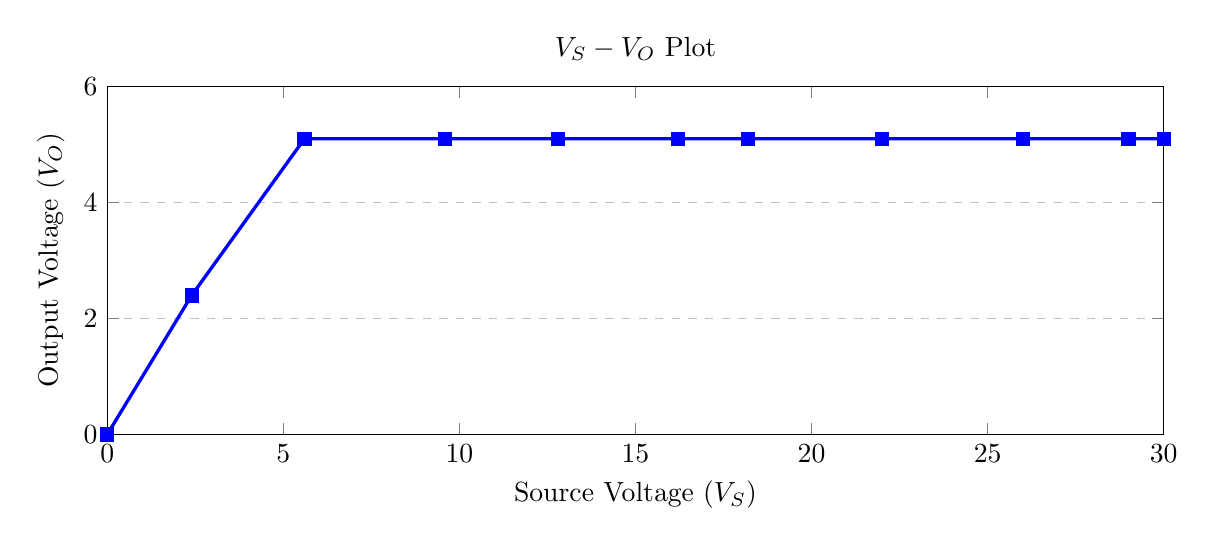
\begin{tikzpicture}
					\begin{axis}[
						title={$V_S - V_O$ Plot},
						width=15cm, height = 6cm,
						xlabel={Source Voltage ($V_S$)},
						ylabel={Output Voltage ($V_O$)},
						xmin=0, xmax=30,
						ymin=0, ymax=6,
						xtick={0,5,10,15,20,25,30},
						ytick={0,2,4,6},
						legend pos=north west,
						ymajorgrids=true,
						grid style=dashed,
%						legend entries = {Forward Biased Silicon Diode}
						]
						
						\addplot[
						color=blue,very thick, mark = square*
						]
						coordinates {
							(0, 0)
							(2.4, 2.4)
							(5.6, 5.10)
							(9.6, 5.10)
							(12.8, 5.10)
							(16.2, 5.10)
							(18.2, 5.10)
							(22, 5.10)
							(26, 5.10)
							(29, 5.10)
							(30, 5.10)
						};					
					\end{axis}
				\end{tikzpicture}
				\caption{$V_S - V_O$ Plot of Zener Diode - LINE Regulator}
			\end{figure}
		
		\newpage
		\subsection{Zener Diode - Load Regulator}
			Zener Voltage ($V_{Z}$): $5.1 V$\\
			Series Resistance($R_{S}$): $0.1 K\Omega$\\
			DC Voltage ($V_{DC}$): $6 V$
			
			\begin{figure}[h!]
				\begin{longtable}[]{@{}llllll@{}}
					\toprule
					Sr No. & Load & Load & Zener & Regulated & \% Voltage\tabularnewline
					& Resistance & Current & Current & Output Voltage & Regulation\tabularnewline
					& ($R_L$) ($\Omega$) & ($I_L$) (mA) & ($I_Z$)(mA) & ($V_O$) (V) & \tabularnewline
					\midrule
					\endhead
					1 & 150 & 34.0 & 0 & 6 & 40.0\tabularnewline
					2 & 266 & 19.2 & 0 & 6 & 27.3\tabularnewline
					3 & 395 & 12.9 & 0 & 6 & 20.2\tabularnewline
					4 & 505 & 10.1 & 0 & 6 & 16.5\tabularnewline
					5 & 609 & 8.37 & 0.626 & 5.10 & 14.1\tabularnewline
					6 & 749 & 6.81 & 2.19 & 5.10 & 11.8\tabularnewline
					7 & 865 & 5.90 & 3.10 & 5.10 & 10.4\tabularnewline
					8 & 969 & 5.26 & 3.74 & 5.10 & 9.35\tabularnewline
					9 & 1073 & 4.75 & 4.25 & 5.10 & 8.53\tabularnewline
					10 & 1195 & 4.27 & 4.73 & 5.10 & 7.72\tabularnewline
					11 & 1250 & 4.08 & 4.92 & 5.10 & 7.41\tabularnewline
					\bottomrule
				\end{longtable}
				\caption{Zener Diode Load Regulator Observations}
			\end{figure}
			\newpage
			\begin{figure}[h]
				\centering
				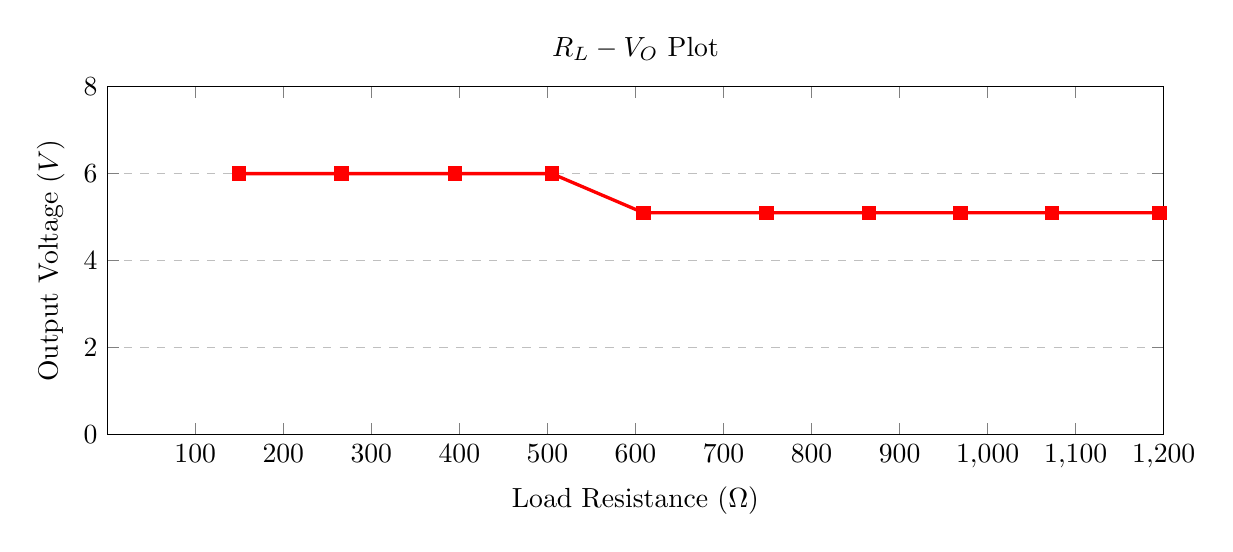
\begin{tikzpicture}
					\begin{axis}[
						title={$R_L - V_O$ Plot},
						width=15cm, height = 6cm,
						xlabel={Load Resistance ($\Omega$)},
						ylabel={Output Voltage ($V$)},
						xmin=0, xmax=1200,
						ymin=0, ymax=8,
						xtick={100,200,300,400,500,600,700,800,900,1000,1100,1200},
						ytick={0,2,4,6,8},
						legend pos=north west,
						ymajorgrids=true,
						grid style=dashed,
						%						legend entries = {Forward Biased Silicon Diode}
						]
						
						\addplot[
						color=red,very thick,mark = square*
						]
						coordinates {
							(150, 6)
							(266, 6)
							(395, 6)
							(505, 6)
							(609, 5.10)
							(749, 5.10)
							(865, 5.10)
							(969, 5.10)
							(1073, 5.10)
							(1195, 5.10)
							(1250, 5.10)
						};					
					\end{axis}
				\end{tikzpicture}
				\caption{$R_L - V_O$ Plot of Zener Diode - LOAD Regulator}
			\end{figure}
		\subsection{Zener Characteristics}			
			\begin{figure}[h]
				\begin{longtable}[]{@{}lll@{}}
					\toprule
					Sr No. & Zener Voltage (V) & Current (mA)\tabularnewline
					\midrule
					\endhead
					1 & 0.120 & 0.000\tabularnewline
					2 & 1.911 & 0.000\tabularnewline
					3 & 3.620 & 0.000\tabularnewline
					4 & 4.724 & 0.001\tabularnewline
					5 & 6.354 & 0.002\tabularnewline
					\bottomrule
				\end{longtable}
				\caption{Zener Diode Characteristics}
			\end{figure}
		
			\begin{figure}[h]
				\centering
				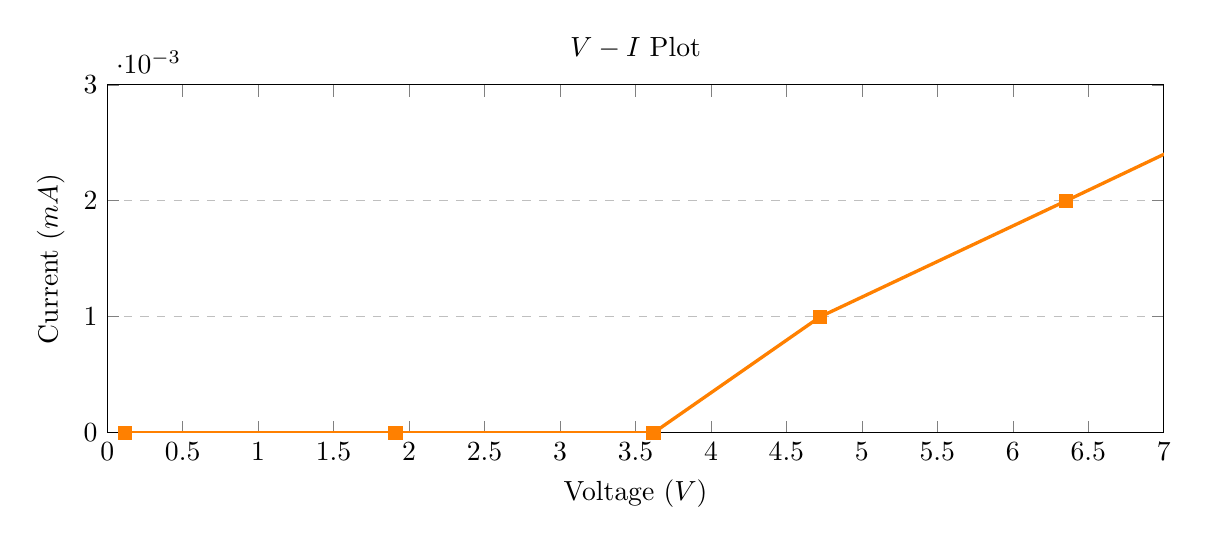
\begin{tikzpicture}
					\begin{axis}[
						title={$V - I$ Plot},
						width=15cm, height = 6cm,
						xlabel={Voltage ($V$)},
						ylabel={Current ($mA$)},
						xmin=0, xmax=7,
						ymin=0, ymax=0.003,
						xtick={0,0.5,1,1.5,2,2.5,3,3.5,4,4.5,5,5.5,6,6.5,7},
						ytick={0,0.001,0.002,0.003},
						legend pos=north west,
						ymajorgrids=true,
						grid style=dashed,
						%						legend entries = {Forward Biased Silicon Diode}
						]
						
						\addplot[
						color=orange,very thick,mark = square*
						]
						coordinates {
							(0.120, 0)
							(1.911, 0)
							(3.620, 0)
							(4.724, 0.001)
							(6.354, 0.002)
							(7.969, 0.003)
							(9.100, 0.006)
						};					
					\end{axis}
				\end{tikzpicture}
				\caption{$V - I$ Plot of Zener Characteristics}
			\end{figure}
		
		\section{Result}
			A Zener Diode is a special kind of diode which permits current to flow in the forward direction as normal, but will also allow it to flow in the reverse direction when the voltage is above the breakdown voltage or ‘zener’ voltage. Zener diodes are designed so that their breakdown voltage is much lower e.g. 2.4 Volts.